\documentclass{prettytex/ox/mmsc-special-topic}

\setlength{\headheight}{19.53pt}
\setlength{\headsep}{1.8em}
\setlength{\belowcaptionskip}{-12pt}
\setminted{fontsize=\footnotesize}
\AfterEndEnvironment{minted}{\vspace*{-0.8cm}}
\renewcommand{\operatorcolor}{black}

\addbibresource{sources.bib}
\tikzexternalize[prefix=tikz/]

\newcommand{\topictitle}{Battery Computing}
\newcommand{\candidatenumber}{1072462}
\newcommand{\course}{Scientific Computing}

\title{\topictitle}
\author{Candidate \candidatenumber}
\date{\today}

\makenoidxglossaries
\newacronym{pde}{PDE}{Partial Differential Equation}
\newacronym{ode}{ODE}{Ordinary Differential Equation}

% TODO: verify oxidation reaction
% TODO: check that all \cL{...} are used on mappings and not values

\begin{document}
  \pagestyle{plain}
  \mmscSpecialHeader[casestudy]

  \begin{abstract}
    \label{abstract}
    This work shall attempt to
    \vspace*{0.2cm}

    \noindent
    \textbf{Our Goal:}
    Numerically obtain the solution $\{a(x, T), b(x, T)\}$ of
    \vspace*{-0.2cm}
    \begin{subequations}
      \begin{empheq}[left={\empheqlbrace}]{align}
        \label{eq:problem-pde-a} &\frac{\partial a}{\partial t} = D_a \frac{\partial^2 a}{\partial x^2}, & a: \R^+ \times [0, T] \mapsto [0, 1],\, T \in \R^+,\; D_a \in \R^+, \\
        \label{eq:problem-pde-b} &\frac{\partial b}{\partial t} = D_b \frac{\partial^2 b}{\partial x^2}, & b: \R^+ \times [0, T] \mapsto [0, 1],\, D_b \in \R^+,               \\
        \label{eq:problem-bcs} &a(\infty, t) = 1,\; b(\infty, t) = 0,                                  & \text{boundary conditions } \forall\, t \in [0, T]\,,               \\
        \label{eq:problem-ics} &a(x, 0) = 1,\;\; b(x, 0) = 0,                                          & \text{initial conditions }\forall\, x \in (0, \infty)\,,            \\
        \label{eq:problem-mass-conservation} &\frac{\partial a}{\partial x} + D \frac{\partial b}{\partial x} = 0 \,, &
      \end{empheq}
    \end{subequations}
    and optionally, $a(0, t) = 0$, which corresponds to \underline{Chronoamperometry} or $\frac{\partial a}{\partial x}\big|_{x=0} = I(t)$ which is set according to a special \underline{Linear Sweep Voltammetry} method with $I(t)$ given by \Cref{eq:current}.
    \vspace*{0.05cm}

    The implementation bla bla
  \end{abstract}

  \begin{figure}[H]
    \centering
    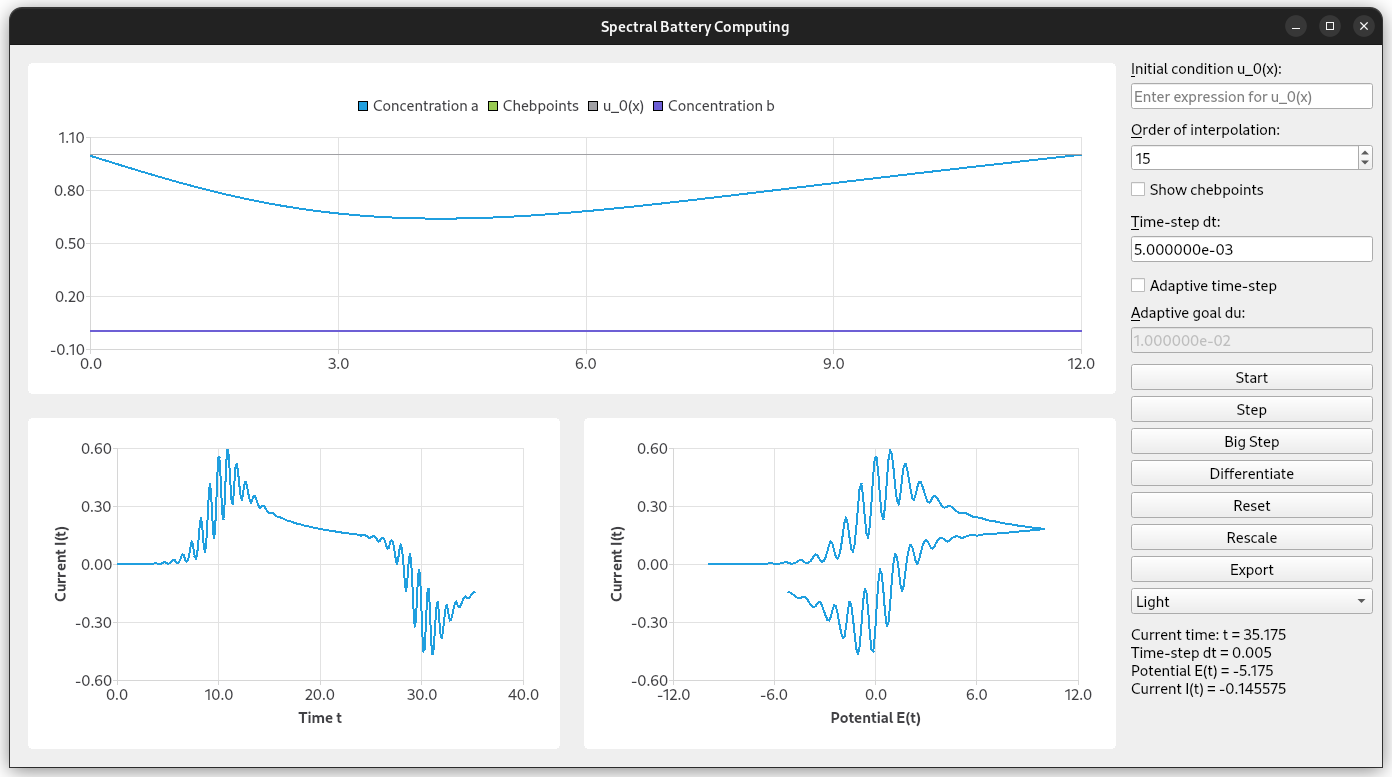
\includegraphics[width=\linewidth]{figures/screenshot.png}
    \caption{Graphical User Interface}
  \end{figure}

  \pagebreak
  \pagestyle{normal}

  \tableofcontents
  \pagebreak

  \section{Problem Introduction}
  Energy storage and its associated challenges are clearly among the most relevant questions, not only for the industrial but also the private sector.
  Politically, many nations in the world are steering towards greener energy supplies.
  Renewable energy sources such as wind and sun usually have a fundamental issue however, their availability is subject to an immense amount of fluctuation, which the energy grid must compensate through short- and long-term energy storage.

  Long-term solutions include for example pumped-storage hydroelectricity facilities, but these must be complemented with short-term storage approaches such as Lithium-Ion or Lithium-Iron-Phosphate ($\text{LiFePO}_4$) batteries.
  Most modern batteries exploit electrochemical reactions to relate electrical potentials with chemical potentials and their associated difference ($\rightarrow$ voltage) and convert energy accordingly.
  The oxidation reaction we considere here is
  $$A \Rightarrow B + e^-?$$
  where $A$ and $B$ can be any chemicals and $e^-$ is an electron \parencite{Gavaghan2000Jan}.

  More bla bla later on.

  \begin{figure}[H]
    \centering
    \inputtikz{battery-schema}
    \caption{Wohoo.}
    \label{fig:battery-schema}
  \end{figure}

  As stated on \Cpageref{abstract}, we consider the following \gls{pde}s in the concentrations $a, b \in \C^2(\Omega)$
  \begin{align}
    \label{eq:pde-a} \frac{\partial a}{\partial t} = D_a \frac{\partial^2 a}{\partial x^2} \\
    \label{eq:pde-b} \frac{\partial b}{\partial t} = D_b \frac{\partial^2 b}{\partial x^2}
  \end{align}

  \subsection{Chronoamperometry}
  \subsection{Linear Sweep Voltammetry}
  \begin{equation}
    I(t) = \kappa_0 \left(a \e^{(1-\alpha) (E(t) - E_0)} - b \e^{-\alpha (E(t) - E_0)}\right)_{x=0}
    \label{eq:current}
  \end{equation}

  \subsection{Linear Sweep AC Voltammetry}
  \begin{equation}
    E(t) = E_{dc}(t) + \Delta E \sin(\omega t)\,.
    \label{eq:ac-potential}
  \end{equation}

  \section{Mathematical Background}
  Let $\N$ denote the nonnegative integers, so $0 \in \N$.
  Similarly, let $\R^+ = [0, \infty)$ denote the nonnegative real numbers.

  \subsection{Laplace Integral Transform}
  What is Laplace?

  \begin{definition}{Laplace Integral Transform}{laplace}
    Given a function $a: \R \mapsto \R$, its Laplace transform $\hat{a}: \C \mapsto \C$ is given by
    $$\hat{a}(s) = \cL\{a\}(s) = \int_{0}^{\infty} a(t) \e^{-st} \,\ddt\,.$$
  \end{definition}

  A notation commonly employed in the context of signal processing is $a(t) \;\laplace\; \hat{a}(s)$ to signify a \textit{transformation pair}, so
  $$a(t) \;\laplace\; \hat{a}(s) \quad\Longleftrightarrow\quad \hat{a}(s) = \cL\{t \mapsto a(t)\}(s)\,.$$
  In the following, we will mostly consider functions of two variables $a: \R \times \R \mapsto \R$ (the concentration of a chemical being a function of time $t \in \R$ and space $x \in \R$).
  In these cases, we are only transforming in one variable, namely $t$, and we will consider $x$ only as a parameter of the transformation pair.

  Laplace transforms are especially valuable for physical systems as many of them expose exponentially decaying and/or periodic behaviours which the Laplace transform is well-suited for due to the form of its kernel.
  Decaying behaviour is captured by the real component of the argument $s$, $\Re(s)$, whereas periodicities are captured by the imaginary part $\Im(s)$\footnote{Consider for comparision the Fourier transform $\cF(a)(\omega) := \int_{-\infty}^{\infty} a(t) \e^{\i \omega t} \,\ddt$ which captures periodic frequencies, where the kernel automatically follows multiplication along the unit circle due to the imaginary-valued exponent $\i\omega t$ (the argument $\omega \in \R$ is real-valued). Intuitively, the Laplace transform coincides with the Fourier transform if evaluated at $s = \i \omega$.}.

  \begin{theorem}{Laplace Transform of the Derivative}{laplace-diff}
    Given a function $a(t)$ and a corresponding Laplace-transform $\hat{a}(s) = \cL\{a\}(s)$, the transform of the derivative $a'(t)$ of the original function is given by
    $$\cL\{a'\}(s) = \cL\left\{t \mapsto \frac{\partial a}{\partial t}\right\}(s) = s\hat{a}(s) - a_0\,,$$
    where $a_0 := a(t=0)$.
  \end{theorem}

  \begin{proof}
    Proof for Laplace's differentiation theorem.
  \end{proof}

  \begin{theorem}{Initial Value}{initial-value}
    For a function $a \in \cC^2(\Omega)$ with corresponding Laplace-transform $\hat{a} = \cL\{a\}$,
    $$\lim_{s \rightarrow \infty} s \hat{a}(s) = \lim_{t \rightarrow 0^+} a(t)$$
    relates $a$'s \textit{initial value} with the transform evaluated at $s \rightarrow \infty$.
  \end{theorem}

  \begin{theorem}{Laplace Convolution}{convolution-theorem}
    For a function $a \in \cC^2(\Omega)$ with corresponding Laplace-transform $\hat{a} = \cL\{a\}$,
    $$\lim_{s \rightarrow \infty} s \hat{a}(s) = \lim_{t \rightarrow 0^+} a(t)$$
    relates $a$'s \textit{initial value} with the transform evaluated at $s \rightarrow \infty$.
  \end{theorem}

  \subsection{Chebyshev Polynomials}
  \begin{definition}{Chebyshev Polynomial of the First Kind}{chebpoly}
    \chebyshev\footnote{Named after Pafnuty Lvovich \chebyshev, alternatively transliterated as Tchebycheff, Tchebyshev (French) or \textsc{Tschebyschow} (German).} polynomials $T_k: \R \mapsto \R$ are functions satisfying
    \begin{align*}
      T_k(x) = T_k(\cos \theta) := \cos(k \theta) = \frac{1}{2} (z^k + z^{-k}) \\
      z := \e^{i \theta},\quad x := \Re(z) = \cos(\theta) = \frac{1}{2}(z + z^{-1})
    \end{align*}
    for degree $k \in \N$. Then, $T_0(x) = 1$, $T_1(x) = x$, $T_2(x) = 2x^2-1$, and so on.
  \end{definition}

  \begin{definition}{Chebyshev Polynomial of the Second Kind}{chebpoly2ndkind}
    Chebyshev polynomials $U_k: \R \mapsto \R$ are functions satisfying
    \begin{align*}
      U_k(\cos \theta) \sin \theta := \sin\left((k+1) \theta\right)
    \end{align*}
    for degree $k \in \N$. Then, $U_0(x) = 1$, $U_1(x) = 2x$, $U_2(x) = 4x^2-1$, and so on.
  \end{definition}
  Note that Chebyhsev polynomials of the first and second kind fulfill the same recurrence relationship, $T_{k+1}(x) = 2x T_k(x) - T_{k-1}(x)$ and $U_{k+1}(x) = 2x U_k(x) - U_{k-1}(x)$. The difference between them arises from the second polynomial respectively which is $T_1(x)=x$ for the first kind and $U_1(x) = 2x = 2 T_1(x)$ for the second kind.

  Proof of $U_k(-1)$'s value.

  \section{Finite Differences}
  Construct $A \vec{x} = \vec{b}$.
  $$\frac{U_{j}^{(n+1)} - U_{j}^{(n)}}{\Delta t} = \alpha \frac{U_{j+1}^{(n)} - 2 U_{j}^{(n)} + U_{j-1}^{(n)}}{(\Delta x)^2}, \quad U_j^{(0)} = u_0(x_j)$$

  \begin{figure}[H]
    \centering
    \inputtikz{fd-scheme}
    \caption{Schematic of the finite different scheme where ... are the nodes specified by initial conditions, and ... are the nodes specified by boundary conditions.}
    \label{fig:fd-scheme}
  \end{figure}

  \subsection{Results}

  \section{Analytical Approaches}
  When $D = 1$, $a + b = 1$ because. % TODO

  \subsection{Similarity Solution}
  The diffusion equations \Cref{eq:problem-pde-a} and \Cref{eq:problem-pde-b} can be solved independently through a similarity solution approach.
  The idea behind the latter is to turn the \gls{pde} into an \gls{ode} by introducing a variable $\eta \in \R$ that depends on both other variables $x$ and $t$.
  For a diffusion-type equation, the correct ansatz would be letting
  $$a(x, t) = f(\eta), \quad \eta := \frac{x}{\sqrt{t}}\,,$$
  with $f: \R \mapsto \R$ and substituting back into \Cref{eq:problem-pde-a} accordingly.
  Respecting the chain rule on derivatives of $f$ accordingly, we arrive at
  $$\frac{\partial a}{\partial t} = -\frac{1}{2} x t^{-\frac{3}{2}} f'(\eta) = D_a \frac{\partial^2 a}{\partial x^2} = D_a t^{-1} f''(\eta)$$
  where we multiply both sides by $t$ to arrive at a simple form
  \begin{align}
    \label{eq:similarity-solution-ode} D_a f''(\eta) + \frac{1}{2} \eta f'(\eta) & = 0\,,
  \end{align}
  which can be solved by substituting $h(\eta) := f'(\eta)$ and solving $D_a \frac{\dd h}{\dd \eta} = \frac{-1}{2} \eta h(\eta)$ by separation of variables:
  $$\int\frac{\dd h}{h} = \frac{-1}{2D_a} \int \eta \,\dd\eta \quad \Rightarrow \quad \ln(h) = -\frac{\eta^2}{4D_a} + \tilde{c_1} \quad\Rightarrow\quad h(\eta) = c_1 \e^{\frac{-1}{4D_a}\eta^2}\,,$$
  which in turn may be integrated to get $f(\eta)$ and thereby $a(x, t)$,
  $$f(\eta) = c_1 \int \e^{\frac{-1}{4D_a}\eta^2} \dd\eta = c_1 \sqrt{D_a \pi} \erf\left(\frac{\eta}{2 \sqrt{D_a}}\right) + c_2\,.$$
  Substituting back, we get
  \begin{align}
    a(x, t) & = c_1 \sqrt{D_a \pi} \erf\left(\frac{x}{2 \sqrt{D_a x}}\right) + c_2\,, \\
    b(x, t) & = c_3 \sqrt{D_b \pi} \erf\left(\frac{x}{2 \sqrt{D_b x}}\right) + c_4\,,
  \end{align}
  where the solution of $b(x, t)$ is obtained by the same procedure.
  Using \Cref{eq:problem-bcs} and \Cref{eq:problem-ics} one can determine $$c_2 = 1 - \sqrt{D_a \pi} c_1\quad \text{ and }\quad c_4 = -\sqrt{D_b \pi} c_3\,.$$
  The spatial derivatives are given by
  $$\frac{\partial a}{\partial x} = c_1 \e^{-\frac{x^2}{4D_at}} t^{-\frac{1}{2}} \quad \text{ and }\quad \frac{\partial b}{\partial x} = c_3 \e^{-\frac{x^2}{4D_bt}} t^{-\frac{1}{2}}\,.$$
  Further considering the mass conservation equation $\frac{\partial a}{\partial x} + D \frac{\partial b}{\partial x} = 0$ (\Cref{eq:problem-mass-conservation}) which couples $a$ with $b$, one can derive a relation between $c_1$ and $c_3$,
  $$c_3 = -\frac{D_a}{D_b} \e^{\left(\frac{1}{D_b} - \frac{1}{D_a}\right) \frac{x^2}{4t}} c_1 = -\frac{D_a}{D_b} \e^{\frac{(D_a-D_b) x^2}{4t D_a D_b}} c_1\,.$$

  In the case of \underline{Chronoamperometry}, the constant $c_1$ is determined by letting
  $$a(x=0, t) = 0 \quad\Rightarrow\quad c_2 = 1 - \sqrt{D_a\pi} c_1 = 0 \quad\Rightarrow\quad c_1 = \frac{1}{\sqrt{D_a \pi}}\,,$$
  whereas for \underline{Linear Sweep Voltammetry} it is determined by
  $$\frac{\partial a}{\partial x}\bigg|_{x=0} = I(t) \quad\Rightarrow\quad c_1 = \sqrt{t} I(t) \text{ and } c_2 = 1 - \sqrt{D_a \pi t} I(t)\,.$$

  % TODO: maybe write down the full expressions? Is maths correct?
  % TODO: When $D = 1$, we have ...

  \subsection{Voltammetry Integral Equation}
  \subsubsection{Derivation using the Laplace Transform}
  As mentioned above, the Laplace Integral Transform is especially useful in the context of differential equations, mostly due to \Cref{thm:laplace-diff}.
  Applying it to our \textit{partial} differential diffusion equation \Cref{eq:pde-a} transforms the problem into one of solving an \textit{ordinary} differential equation.
  Similarly, \glstext{ode}s could be turned into algebraic equations using a similar approach.

  Starting from \Cref{eq:pde-a}, we Laplace-transform both sides and then apply \Cref{thm:laplace-diff} in time $t$ to arrive at
  \begin{align*}
    \frac{\partial a}{\partial t}                                   & = D_a \frac{\partial^2 a}{\partial x^2} \quad                             & \textcolor{gray}{\text{Laplace-transform w.r.t. } t} \\
    \cL\left\{t \mapsto \frac{\partial a}{\partial t}\right\}       & = D_a \cL\left\{t \mapsto \frac{\partial^2 a}{\partial x^2}\right\} \quad & \textcolor{gray}{\text{Use \Cref{thm:laplace-diff}}} \\
    s \hat{a}(s) - a_0(x)                                           & = D_a \frac{\partial^2 \hat{a}}{\partial x^2} \quad                       & \textcolor{gray}{\text{Rearrange}}                   \\
    \frac{\partial^2 \hat{a}}{\partial x^2} - \frac{s}{D_a} \hat{a} & = -\frac{a_0(x)}{D_a}
  \end{align*}
  where $\hat{a} := \cL\{a\}$ and $a_0(x) := a(x, t=0)$, which is a second-order constant-coefficient \glsdesc{ode} in space $x$. Its characteristic polynomial is $\lambda^2 + \frac{s}{D_a} = 0$ which, together with the initial condition $a_0 = 1$ and resulting particular solution $\hat{a}_p(x, s) = \cL\{-1\}(s) = \frac{1}{s}$\footnote{$\cL\{1\} = \int_{0}^{\infty} \e^{-st} \,\ddt = \frac{1}{s} \left[\e^{-st}\right]_0^\infty = \frac{-1}{s}$.}, leads us to the general solution
  \begin{equation}
    \hat{a}(x, s) = c_1 \e^{\sqrt{\frac{s}{D_a}}x} + c_2 \e^{-\sqrt{\frac{s}{D_a}}x} + \frac{1}{s D_a}\,,\quad c_1, c_2 \in \R\,.
    \label{eq:laplace-pre-solution}
  \end{equation}

  The constant $c_1$ then vanishes when applying the initial value theorem (\Cref{thm:initial-value})
  $$\lim_{s \rightarrow \infty} s \hat{a}(s) = \lim_{s \rightarrow \infty} \underbrace{c_1 s \e^{\sqrt{\frac{s}{D_a}}x}}_{\rightarrow \infty} + \underbrace{c_2 s \e^{-\sqrt{\frac{s}{D_a}}x}}_{\rightarrow 0} + 1 \overset{!}{=} \lim_{t \rightarrow 0^+} a(t) = 1$$
  because $c_1 \neq 0$ would cause its corresponding term to explode. Considering the other boundary condition of linear sweep voltammetry
  $$\frac{\partial a}{\partial x}\bigg|_{x=0} = I(t) \quad \Leftrightarrow \quad \frac{\partial \hat{a}}{\partial x} \overset{!}{=} \hat{I}(s) \quad \Leftrightarrow \quad c_2 \sqrt{\frac{s}{D_a}} \e^{0} = \hat{I}(s)\,,$$
  where $\hat{I}(s) := \cL\{I\}(s)$ and we obtain $c_2(s) = \frac{-\hat{I}(s)}{\sqrt{s}}$.
  So \Cref{eq:laplace-pre-solution} becomes
  \begin{equation}
    \hat{a}(x, s) = \frac{-\hat{I}(s)}{\sqrt{s}} \e^{-\sqrt{\frac{s}{D_a}}x} + \frac{1}{s D_a}\,,
    \label{eq:laplace-solution}
  \end{equation}
  which, evaluated at $x = 0$, becomes $\hat{a}(s, 0) = \frac{-\hat{I}(s)}{\sqrt{s}} + \frac{1}{s D_a}$, depending on the Laplace transform of the current $I(t)$.

  In principle, this is already a complete result in and of itself, as it provides the full solution on the entire domain in frequency-space \footnote{Frequency space is a term borrowed from Fourier analysis, where we say that the transformed functions reside in ``frequency space''. The usage is the same for Laplace's transformation.}. If one obtains the Laplace-transform of the current expression \Cref{eq:current} and performs the inverse transform of $\hat{a}$, even just numerically, the linear sweep voltammetry problem is solved in full as a similar procedure leads to the solution of the other concentration $b$.

  \subsubsection{At the Boundary}
  Within the scope of this report, we will consider an integral equation relating current $I(t)$ and the potential $E(t)$ to verify our numerical results.
  Inverse-transforming \Cref{eq:laplace-solution} at $x = 0$ where our boundary condition is given and using the convolution theorem (\Cref{thm:convolution-theorem}), we arrive at
  \begin{align*}
    a(x, t) = -\cL^{-1}\left\{s \mapsto \hat{I}(s) \cdot \hat{g}(s)\right\}(t) + \cL^{-1}\left\{s \mapsto \frac{1}{s D_a}\right\}(t) = -(I * g)(t) + \frac{1}{D_a}\,,
  \end{align*}
  where we introduced $\hat{g}(s) := \frac{1}{\sqrt{s}} = \cL\{g\}(s)$ the Laplace transfrom of $g(t) = \frac{1}{\sqrt{\pi t}}$.
  \begin{proof}
    $\cL\{t \mapsto \frac{1}{\sqrt{\pi t}}\}(s) = \frac{1}{\sqrt{\pi}} \int_0^\infty t^{-\frac{1}{2}} \e^{-st} \,\ddt = \frac{1}{\sqrt{\pi}} \int_0^\infty \cancel{t^{-\frac{1}{2}}} \e^{-su^2} \cancel{t^{\frac{1}{2}}}\,\ddu = \left[\erf(\sqrt{s} u) / \sqrt{s}\right]_0^\infty$ where we used a substitution $u = \sqrt{t}$ to resolve the product in the integrand, resulting in the Gaussian integral and subsequently, the error function $\erf(\sqrt{s}u)$ which satisfies $\erf(0) = 0$ and $\erf(\infty) = 1$ so the full transformation pair is $\frac{1}{\sqrt{\pi t}} \;\laplace\; \frac{1}{\sqrt{s}}$.
  \end{proof}

  \subsubsection{Simplification when $D = 1$ and $\kappa_0 \gg 1$}
  When $D = 1$, this results in the following expressions for $a(x=0, t)$ and $b(x=0, t)$,
  \begin{align}
    \label{eq:laplace-a} a(x=0, t) & = 1 - (I * g)(t) = 1 - \int_{0}^{t} \frac{I(\tau)}{\sqrt{\pi (t - \tau)}} \,\dd\tau\,, \\
    \label{eq:laplace-b} b(x=0, t) & = 1 - a(x=0, t) = \int_{0}^{t} \frac{I(\tau)}{\sqrt{\pi (t - \tau)}} \,\dd\tau\,,
  \end{align}
  which can be even further simplified when considering $\kappa_0 \gg 1$, where from \Cref{eq:current} we have the following relationship of $I(t)$, $E(t)$ and $b_0(t)$
  \begin{align*}
    I(t) & = \kappa_0 (1-b_0) \e^{(1-\alpha) V} - \kappa_0 b_0 \e^{-\alpha V} \\
         & = \kappa_0 \left[(1-b_0) \e^V - b_0\right] \e^{-\alpha V}          \\
         & = \kappa_0 \left[\e^V - (1+\e^V) b_0\right] \e^{-\alpha V}
  \end{align*}
  where $V(t) := E(t) - E_0(t)$, $a_0 = a(x=0, t)$ and $b_0 = b(x=0, t)$.
  It can be further rearranged and simplified to yield an approximation to $b_0$,
  \begin{align*}
    \frac{I(t)}{\kappa_0 \e^{-\alpha V}} = \e^V - (1+\e^V) b_0 \quad \Leftrightarrow \quad
    b_0 = \frac{\e^V - \frac{I(t)}{\kappa_0 \e^{-\alpha V}}}{1+\e^V} \approx \frac{\e^V}{1 + \e^V} \quad \text{ when } \kappa_0 \gg 1\,,
  \end{align*}
  which can be combined with \Cref{eq:laplace-b} to obtain
  \begin{equation}
    b_0 = \int_{0}^{t} \frac{I(\tau)}{\sqrt{\pi (t - \tau)}} \,\dd\tau \approx \frac{1}{1+\e^{-V}} \quad \Leftrightarrow \quad \int_{0}^{t} \frac{I(\tau)}{\sqrt{(t - \tau)}} \,\dd\tau \approx \frac{\sqrt{\pi}}{1 + \e^{-(E(t) - E_0)}}\,,
    \label{eq:numerical-verification}
  \end{equation}
  which we will use to numerically verify our results.

  \subsubsection{Numerical Verification}
  Numerically integrating the left-hand side convolution in \Cref{eq:numerical-verification} using a quadrature rule and comparing it with the right-hand side, from the spectral solver we obtain a relatively close match as can be seen in \Cref{fig:voltammetry-convolution}.
  \begin{figure}[H]
    \centering
    \inputtikz{voltammetry-convolution}
    \caption{Convolution Integral: Comparing $\int_{0}^{t} \frac{I(\tau)}{\sqrt{(t - \tau)}} \,\dd\tau$ (in \textcolor{blue}{blue}) with $\frac{\sqrt{\pi}}{1 + \e^{-(E(t) - E_0)}}$ (in \textcolor{green}{green}) for the DC and AC case with parameter $\Delta E = 0.3$ over the DC potential $E_{dc}(t)$. $\kappa_0 = 35$ is chosen large and we further have $\alpha = 0.9$, $E_0 = 0$ and $t_{rev} = 20$.}
    \label{fig:voltammetry-convolution}
  \end{figure}

  \section{Spectral Method}
  The basic idea of a spectral method is to turn a differential equation into an algebraic one by considering a basis expansion ansatz of the form
  \begin{equation}
    f_N(\xi) = \sum_{k=0}^{N-1} a_k T_k(\xi), \quad k \in \{0, ..., N-1\},\quad N \in \N, N > 1\,,
    \label{eq:truncated-cheb-series}
  \end{equation}
  where we choose the basis of Chebyshev polynomials of the first kind.

  An initial condition may be obtained by
  One wishes to interpolate through data points

  \begin{theorem}{Chebyshev series coefficient formula}{cheb-coefficient-integrals}
    For any function $f: [-1, 1] \mapsto \R$, one can obtain the \chebyshev series coefficients $a_k$, $k \in \N$ as
    \begin{align*}
      a_0 & = \frac{1}{\pi} \langle f, T_0 \rangle =  \frac{1}{\pi} \int_0^\pi f(\cos \theta) \dd\theta                                   \\
      a_k & = \frac{2}{\pi} \langle f, T_k \rangle = \frac{2}{\pi} \int_0^\pi f(\cos \theta) \cos(k \theta) \dd\theta, \quad k \neq 0 \,.
    \end{align*}
  \end{theorem}

  Because the domain we are interested in $[0, L]$ as specified in \Cref{eq:problem-pde-a,eq:problem-mass-conservation} is not $[-1, 1]$, we rescale the expansion as follows when evaluating:
  $$f_N(x) = f_N\left(\xi = \frac{2 x}{L} - 1\right)$$
  to get from $x \in [0, L]$ to $\xi \in [-1, 1]$.

  From the definition of Chebyshev polynomials $T_k(x) = \cos(k\theta)$, confer \Cref{def:chebpoly}, we can derive that
  $$\frac{\dd T_k}{\ddx} = \frac{\dd T_k}{\dd\theta} \frac{\dd\theta}{\ddx} = ... = k U_{k-1}(x)\,,$$
  where $U_k: [-1, 1] \mapsto \R$ denote the Chebyshev polynomials of the second kind, $U_k(\cos \theta) \sin(\theta) = \sin\left((n+1) \theta\right)$, confer \Cref{def:chebpoly2ndkind}.

  In order to enforce a von-Neumann boundary condition on the left and a Dirichlet boundary condition on the right,
  we are interested in explicitly setting coefficients $a_k$ such that
  $$a_x(-1, t) = \frac{\dd a}{\ddx}\Big|_{x=-1} = \tilde{l} \quad \text{ and } \quad a(1) = r, \quad \text{ where } \quad \tilde{l}, r \in \R\,.$$

  Using the Chebyshev series ansatz
  $$a(x, t) = \sum_{k=0}^{N-1} a_k^{(t)} T_k(x)$$
  we have that
  $$\frac{\dd a}{\ddx} = \sum_{k=0}^{N-1} a_k^{(t)} \frac{\dd T_k}{\ddx}(x)\,,$$
  so we are interested in
  $$a_x(-1, t) = \frac{\dd a}{\ddx}\Big|_{x=-1} = \sum_{k=0}^{N-1} a_k^{(t)} \frac{\dd T_k}{\ddx}\Big|_{x=-1} = \sum_{k=0}^{N-1} a_k^{(t)} k U_{k-1}(-1)\,.$$

  Following from TODO (explained on Wikipedia), we know that
  $$U_k(-1) = (-1)^k (k+1) \quad \text{ and } \quad T_k(1) = 1 \quad \forall k \in \N\,,$$
  which turns our conditions into algebraic conditions w.r.t. the coefficients $a_k^{(t)}$,
  $$a_x(-1, t) = \frac{\dd a}{\ddx}\Big|_{x=-1} = \sum_{k=0}^{N-1} a_k^{(t)} k^2 (-1)^{k-1} \overset{!}{=} \tilde{l} \quad \text{ and } \quad a|_{x=1} = \sum_{k=0}^{N-1} a_k^{(t)} \overset{!}{=} r\,.$$

  Knowing that the heat equation Forward Euler numerical scheme modifies all but the two highest-degree coefficients in the series, we expand:
  \begin{align*}
    a_x(-1, t) = \sum_{k=0}^{N-1} a_k^{(t)} T_k'(-1) =   & \overbrace{-\sum_{k=0}^{N-3} a_k^{(t)} k^2 (-1)^{k}}^{:= \Sigma_3} - (N-2)^2 (-1)^{N-2} a_{N-2}                  \\
                                                         & -(N-1)^2 (-1)^{N-1} a_{N-1} = l\,,                                                                               \\
    a(1, t)    = \sum_{k=0}^{N-1} a_k^{(t)} T_k(1)     = & \underbrace{\sum_{k=0}^{N-3} a_k^{(t)}}_{:= \Sigma_2}              + a_{N-2}                    + a_{N-1} = r\,,
  \end{align*}

  \subsection{Enforcing Boundary Conditions}
  Von Neumann on the left

  \subsection{Stability and Implicit Euler}

  \subsection{Implementation}
  The solver was implemented in C++, using TschebFun and is based on the HeatFun numerical integrator.

  % \inputminted{cpp}{../SpectralSolver/Solver.h}

  \subsection{Results}
  Chronoamperometry (step potential),

  \begin{figure}[H]
    \centering
    \inputtikz{chronoamperometry}
    \caption{Chronoamperometry}
    \label{fig:chronoamperometry}
  \end{figure}

  DC Linear Sweep Voltammetry,
  AC Linear Sweep Voltammetry

  \begin{figure}[H]
    \centering
    \inputtikz{ac-voltammetry}
    \caption{AC Voltammetry}
    \label{fig:ac-voltammetry}
  \end{figure}

  \begin{figure}[H]
    \centering
    \inputtikz{different-E0s}
    \caption{Voltammetry Current $I(t)$ vs. the DC Potential $E_{dc}(t)$}
    \label{fig:different-E0s}
  \end{figure}

  \begin{figure}[H]
    \centering
    \inputtikz{voltammetry-current}
    \caption{Voltammetry Current $I(t)$ vs. the DC Potential $E_{dc}(t)$}
    \label{fig:voltammetry-current}
  \end{figure}

  \subsection{Convergence behaviour}

  \section{Conclusion}

  \begin{table}[H]
    \caption{Runtime Comparison}
  \end{table}

  \pagebreak
  \printbibliography
  \printnoidxglossary[type=acronym]

  \appendix
  \section{Implementation}
  The results above were obtained using implementations of the numerical methods described.
  Three (independent) solvers are available, in MATLAB and in Python and the spectral solver (cf. the folder named \texttt{SpectralSolver}) which is written in C++.
  All code is available on GitHub, in the \href{https://github.com/MrP01/BatteryComputing}{MrP01/BatteryComputing} repository.
\end{document}
